\documentclass[12pt,UTF8,fleqn]{ctexart}
\usepackage{ctex,amsmath,amssymb,geometry,fancyhdr,bm,amsfonts,mathtools,extarrows,graphicx,url,enumerate,xcolor,float,multicol,wasysym}
\usepackage{subfigure}
\allowdisplaybreaks[4]
% 加入中文支持
\newcommand\Set[2]{\left\{#1\ \middle\vert\ #2 \right\}}
\newcommand\Lim[0]{\lim\limits_{n\rightarrow\infty}}
\newcommand\LIM[2]{\lim\limits_{#1\rightarrow#2}}
\newcommand\Ser[1]{\sum_{n=#1}^\infty}
\newcommand{\SER}[2]{\sum_{#1=#2}^\infty}
\newcommand{\Int}[4]{\varint\nolimits_{#1}^{#2}#3\mathrm d#4}
\newcommand{\aIInt}[1]{\iint\limits_{#1}}
\newcommand{\IInt}[3]{\iint\limits_{#1}#2\mathrm d#3}
\newcommand{\varIInt}[4]{\iint\limits_{#1}#2\mathrm d#3\mathrm d#4}
\newcommand{\IIInt}[3]{\iiint\limits_{#1}#2\mathrm d#3}
\newcommand{\varIIInt}[5]{\iiint\limits_{#1}#2\mathrm d#3\mathrm d#4\mathrm d#5}
\newcommand{\LInt}[3]{\varint\nolimits_{#1}#2\mathrm d#3}
\newcommand{\LOInt}[3]{\varoint\nolimits_{#1}#2\mathrm d#3}
\newcommand{\LLInt}[4]{\varint\nolimits_{#1}\nolimits^{#2}#3\mathrm d#4}
\newcommand{\BLInt}[2]{\varint\nolimits_{#1}#2}
\newcommand{\varBLInt}[3]{\varint\nolimits_{#1}\nolimits^{#2}#3}
\newcommand{\BLOInt}[2]{\varoint\nolimits_{#1}#2}
\newcommand{\SIInt}[3]{\iint\limits_{#1}#2\mathrm d#3}
\newcommand{\md}[1]{\mathrm d#1}
\newcommand{\BSIInt}[2]{\iint\limits_{#1}#2}
\newcommand{\pp}[2]{\frac{\partial #1}{\partial #2}}
\newcommand{\ppx}[1]{\frac{\partial #1}{\partial x}}
\newcommand{\ppy}[1]{\frac{\partial #1}{\partial y}}
\newcommand{\ppz}[1]{\frac{\partial #1}{\partial z}}
\newcommand{\varppx}[1]{\frac{\partial}{\partial x} #1}
\newcommand{\varppy}[1]{\frac{\partial}{\partial y} #1}
\newcommand{\varppz}[1]{\frac{\partial}{\partial z} #1}
\newcommand{\BSOIInt}[2]{\oiint\limits_{#1}#2}
\newcommand{\me}[0]{\mathrm e}
\geometry{a4paper,scale=0.80}
\pagestyle{fancy}
\rhead{常微分方程(1)}
\lhead{基础习题课期末复习}
\chead{微积分B(2)}
\begin{document}
\setcounter{section}{15}
\section{常微分方程的基本概念和初等解法}
\subsection{复习计划}
\begin{figure}[H]
\begin{center}
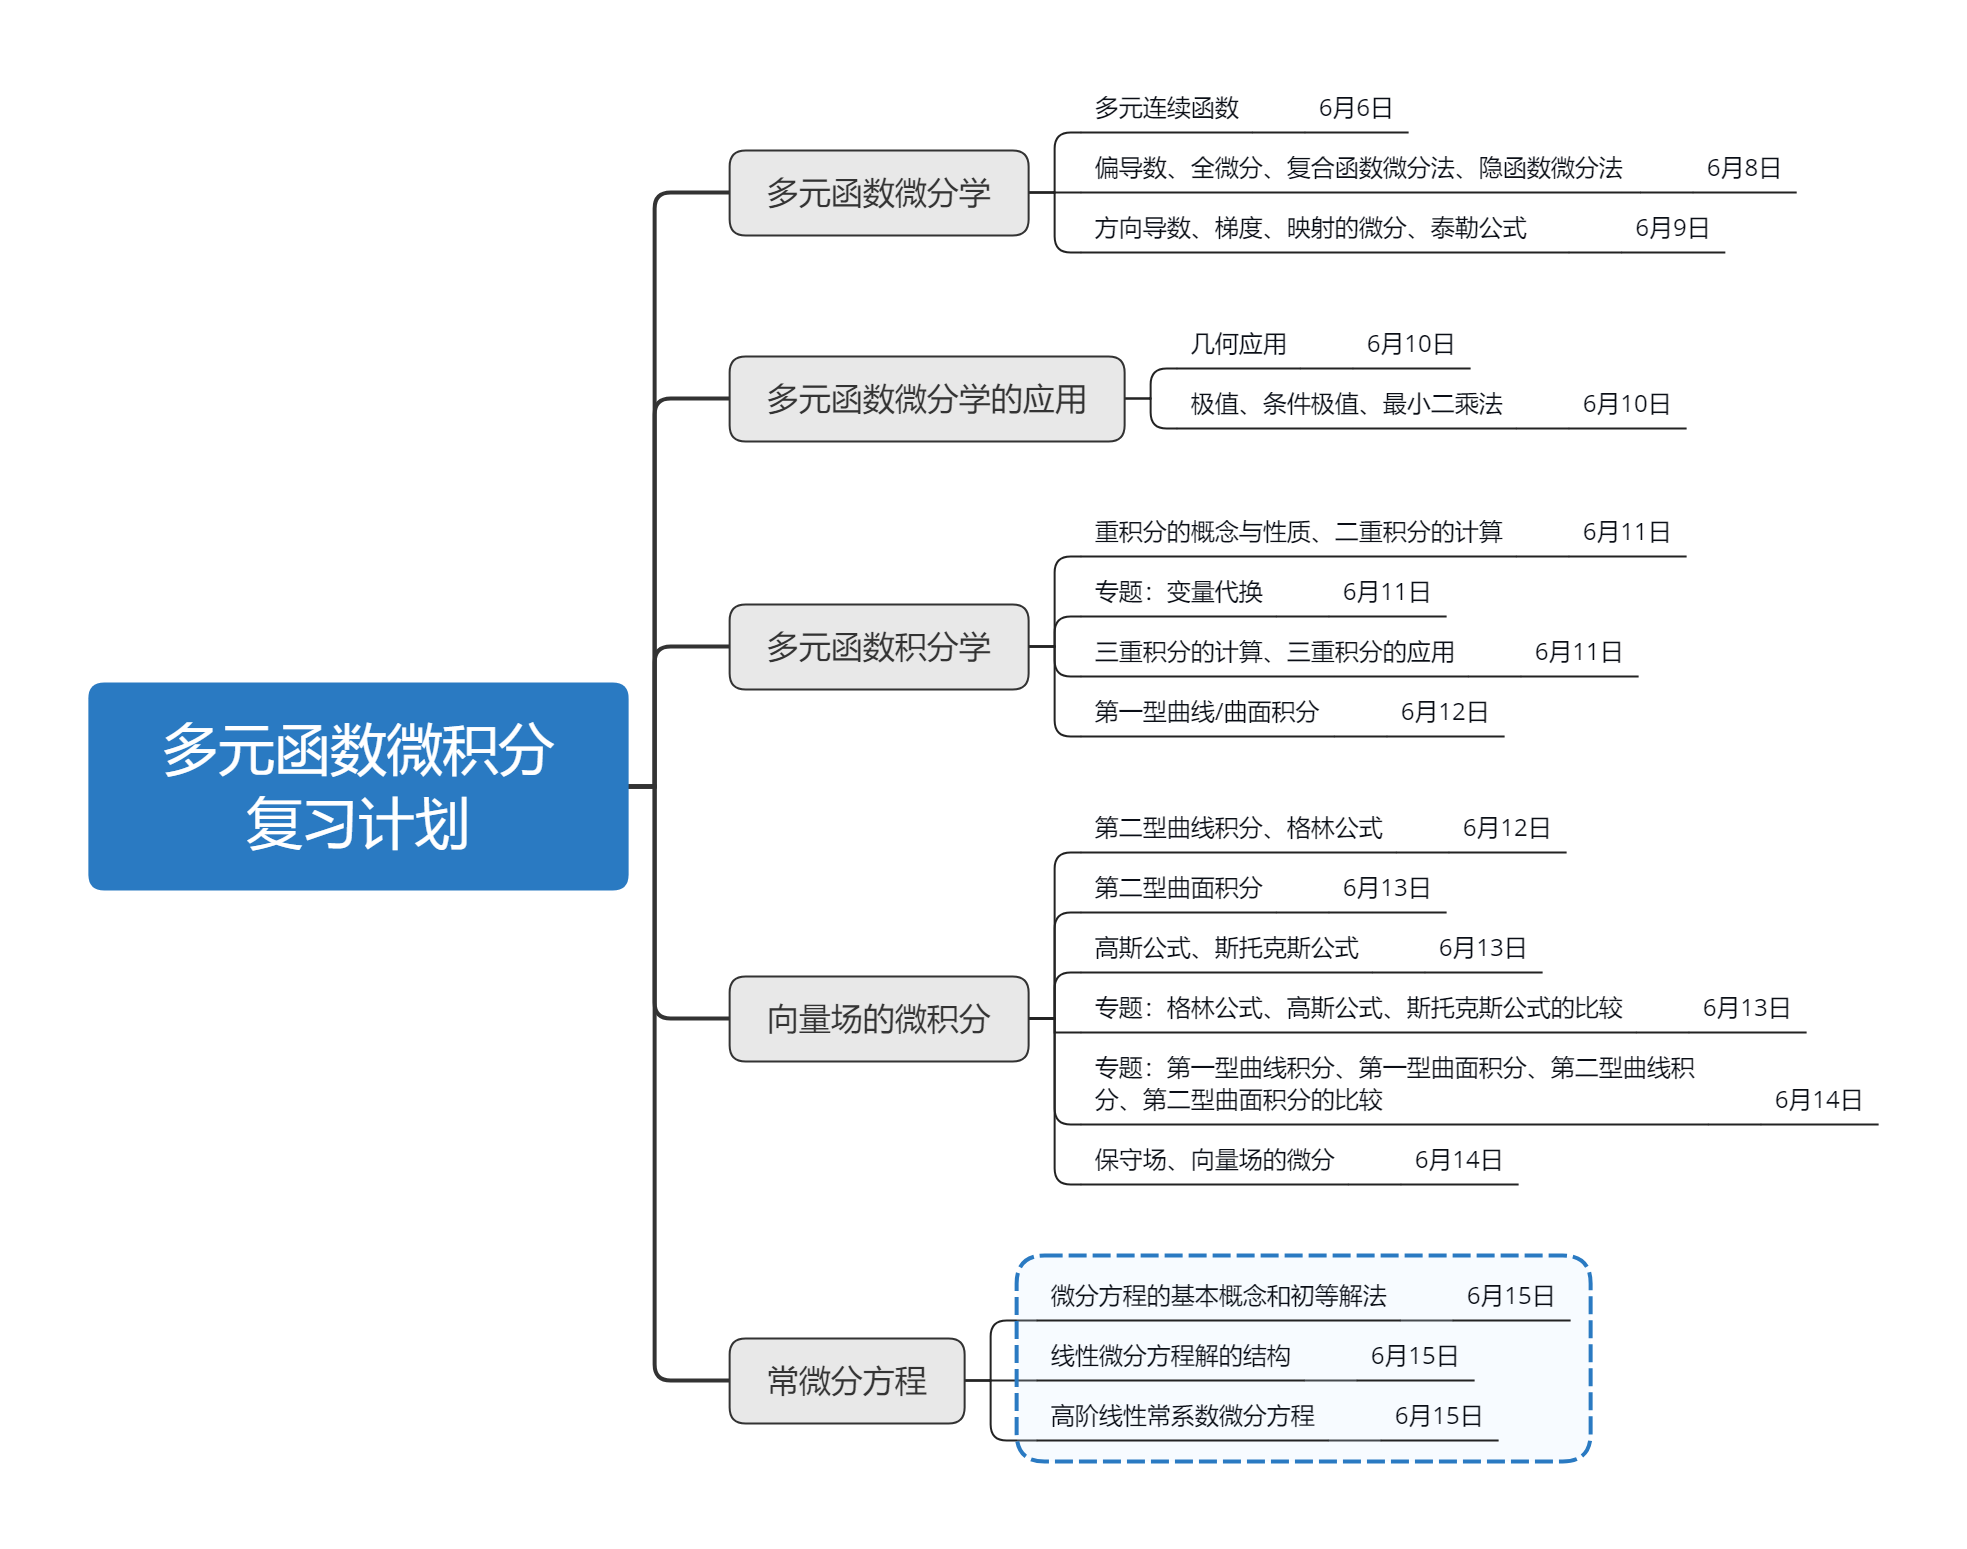
\includegraphics[height=0.5\textheight]{Figures20190615/plan.png}
\end{center}
\end{figure}
\subsection{知识结构}
\begin{figure}[H]
\begin{center}
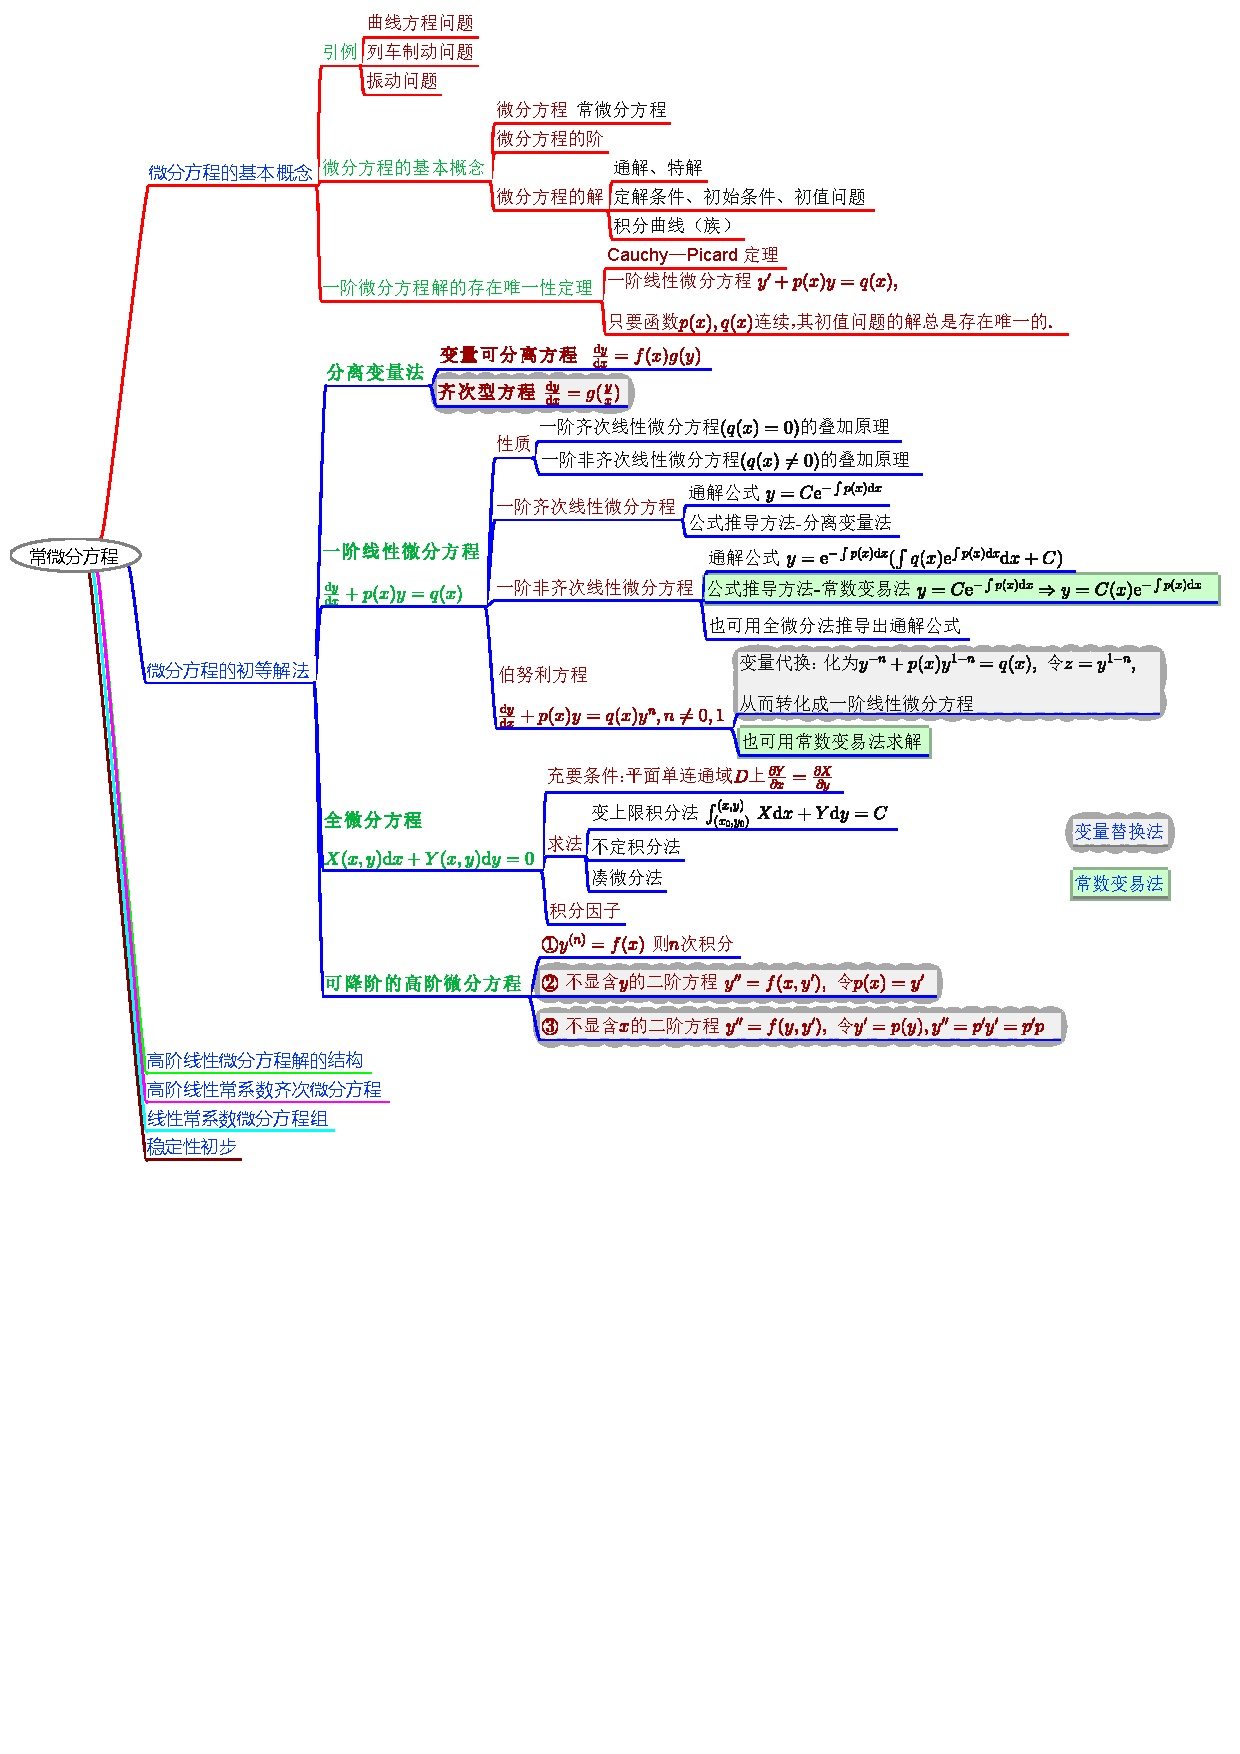
\includegraphics[height=1\textheight]{20190615.pdf}
\end{center}
\end{figure}

\subsection{常微分方程的初等解法}
\begin{enumerate}
\item常微分方程的初等解法:
\begin{figure}[H]
\begin{center}
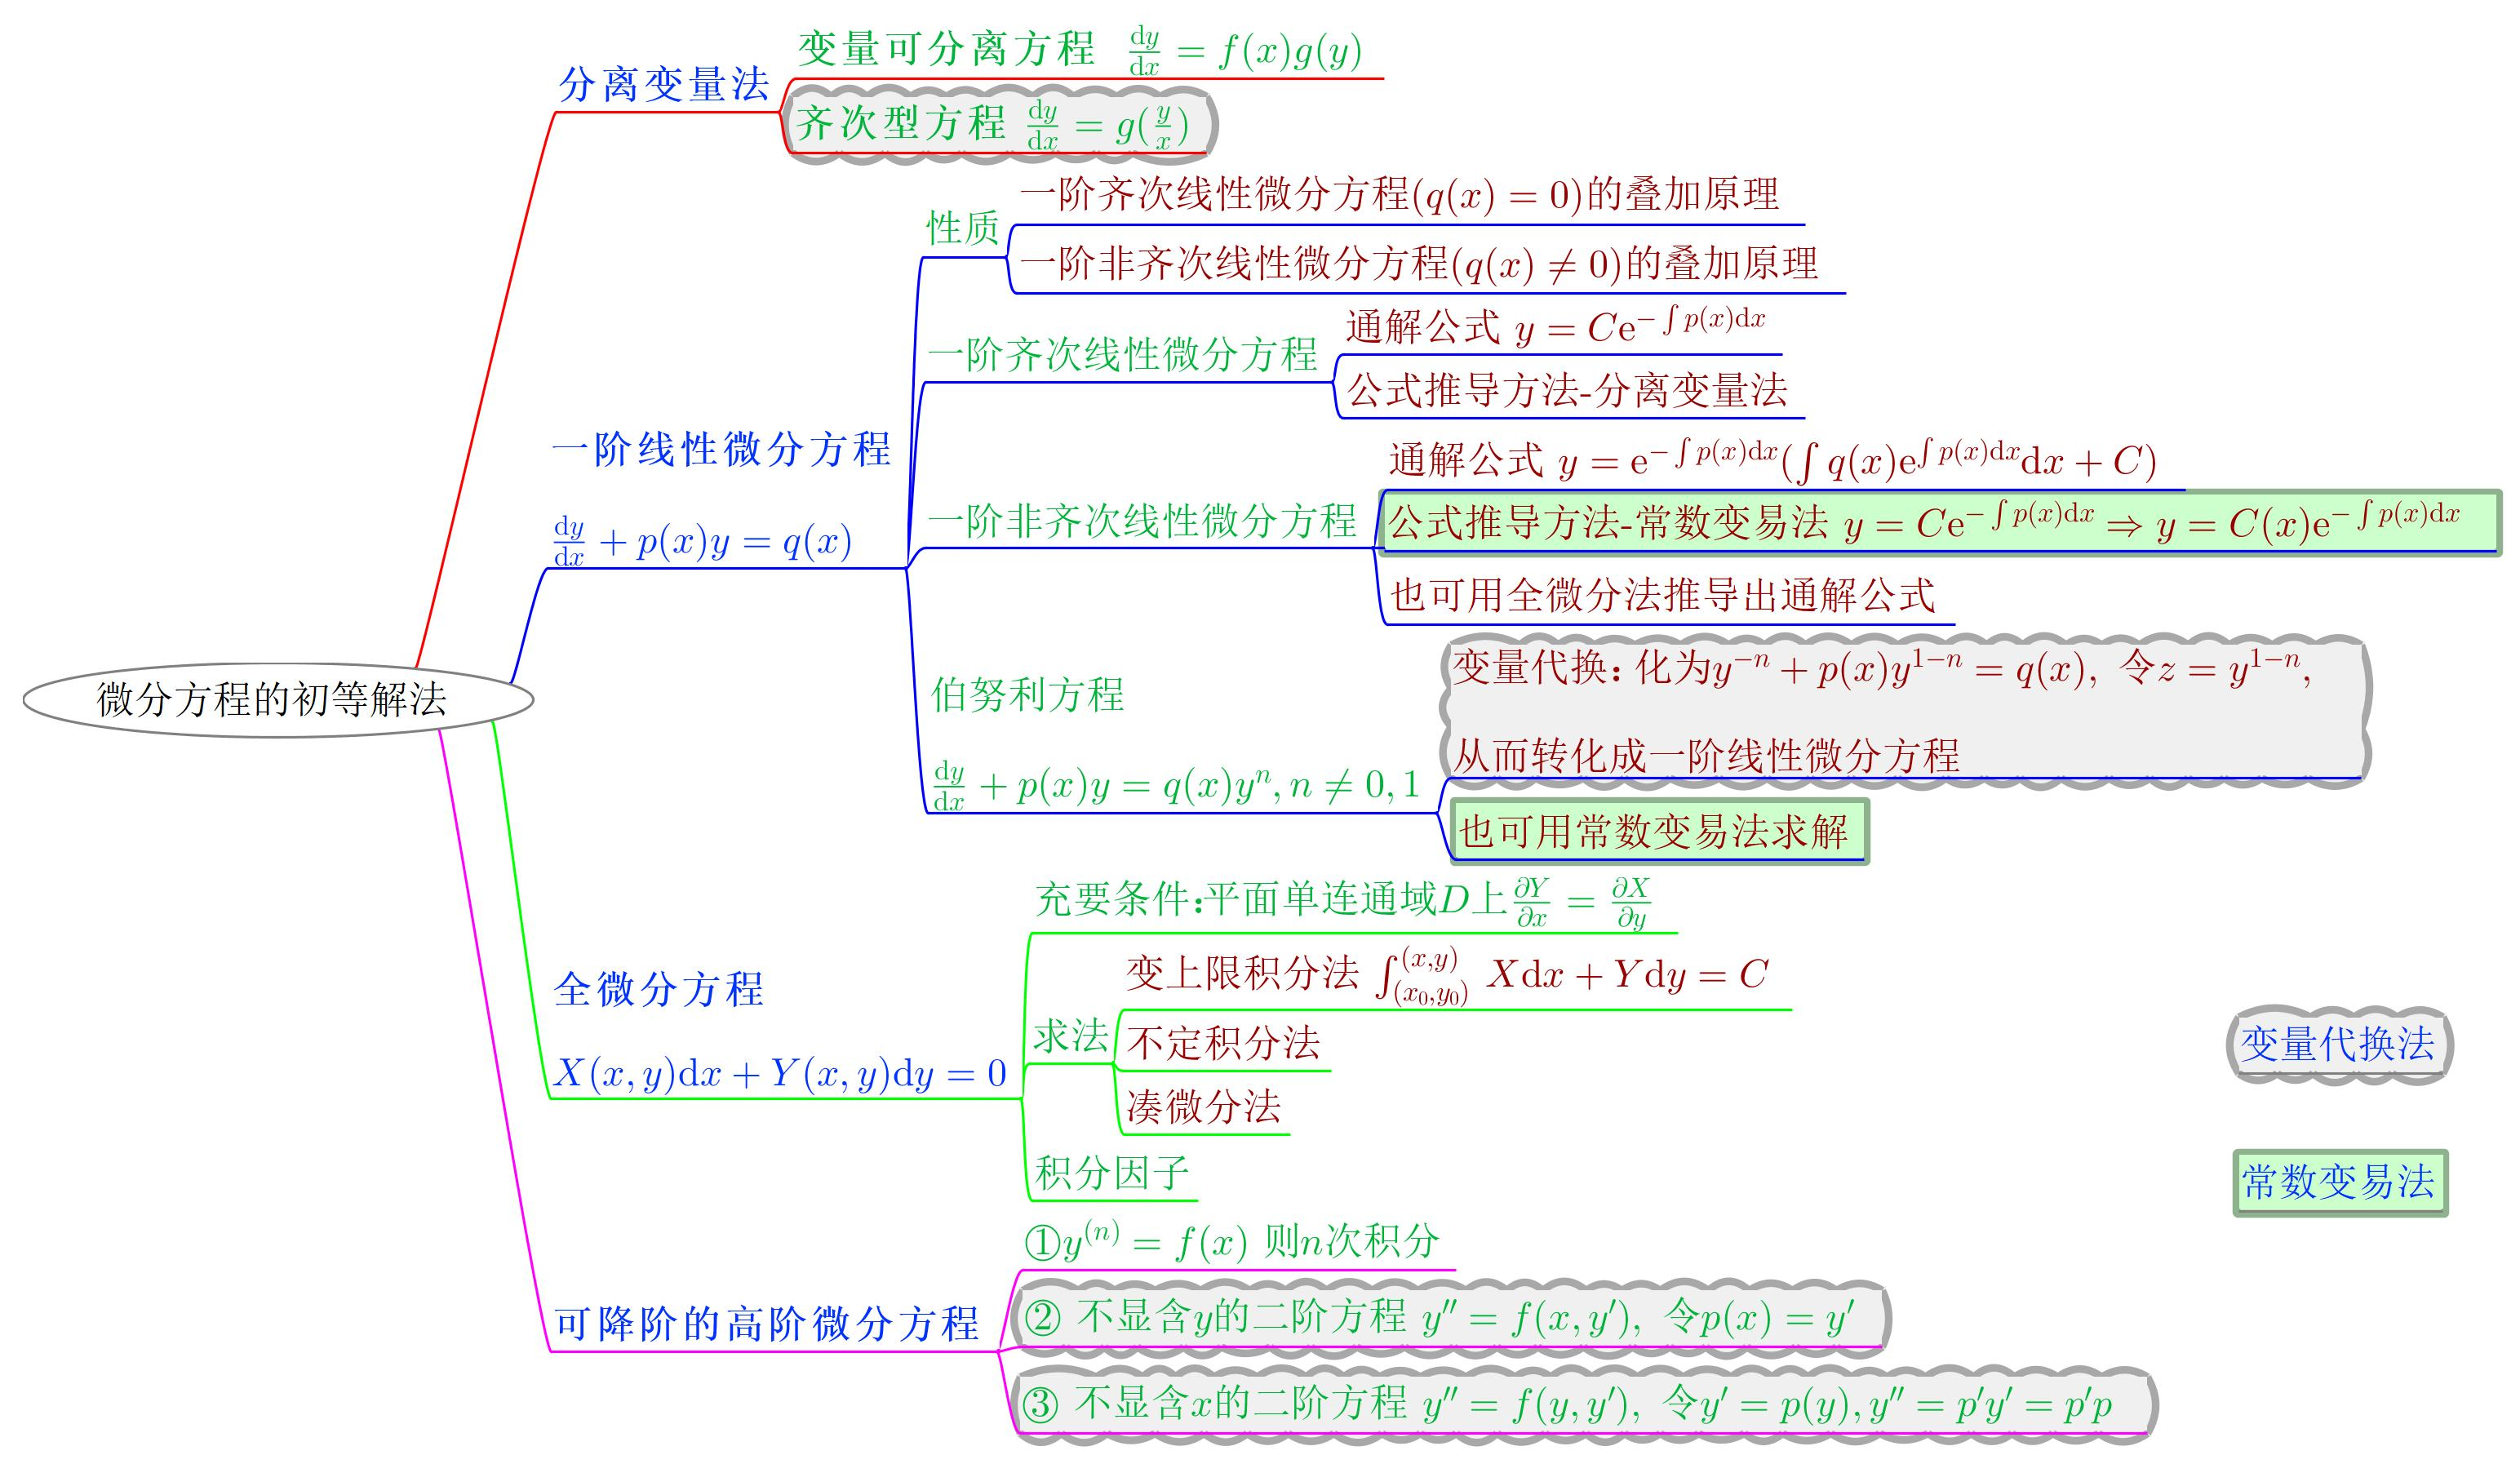
\includegraphics[height=0.45\textheight]{structures.jpg}
\end{center}
\end{figure}

注意:
\begin{enumerate}
\item对于一阶非齐次线性微分方程可直接代入通解公式进行求解,不需先求对应齐次方程的通解再用常数变易法,即不需自行推导该通解公式.
\item变量代换法是求解常微分方程的常用方法.
\item常数变易法(变动任意常数法)也是求解常微分方程的常用方法.
\end{enumerate}
\end{enumerate}
\subsection{习题分类与解题思路}
\begin{enumerate}
\item分离变量法. 分离变量法是十分基本和常用的方法.

【习题14.2中的1.(1)/(2)/(3)/(4)/(5)/(6).】
\item齐次方程.

【习题14.2中的2.(1)/(2)/(3)/(4)/(5)/(6).】

对称形式的微分方程$X\md x+Y\md y=0$经过变形、可降阶的高阶微分方程经过降阶也可能得到齐次方程,可用齐次方程变量代换的方法求解.

【如习题14.2中的5.(4), 7.(3)/(4).】
\item一阶线性非齐次方程. 一阶线性非齐次方程求解的最好方法就是代入通解公式求解.

【习题14.2中的3.(1)/(2)/(3)/(4)/(5)/(6)/(7)/(8)/(9)/(10).】

一阶线性非齐次微分方程通解公式的积分号中可能会出现绝对值,此时可只考虑$x>0$或$x<0$的情况,或者根据初始条件取$x>0$或$x<0$,把绝对值去掉,在结果中标明$x>0$或$x<0$即可.

【如习题14.2中的3.(3)/(6)/(7), 4.(2), 7.(1).】
\item伯努利方程. 伯努利方程的形式大家要记住,处理的方法是变量代换化成一阶线性非齐次微分方程,然后用一阶线性非齐次微分方程的通解公式进行求解.

【如习题14.2中的4.(1)/(2), 6.(1)/(2)/(3).】
\item全微分方程. 遇到了对称形式的微分方程$X\md x+Y\md y=0$,求解思路如下:
\begin{enumerate}
\item[第一步]首先尝试凑微分法,如能利用凑微分法得到原函数,则可直接求解;

【如习题14.2中的5.(2)/(3), 9.】
\item[第二步]如不能利用凑微分法得到原函数,则判断$X\md x+Y\md y=0$是否为全微分方程. 若定义域为平面单连通域且$\ppx Y=\pp yX$,则$X\md x+Y\md y=0$是全微分方程,可应用曲线积分法或不定积分法求原函数.

【如习题14.2中的5.(1).】
\item[第三步]如定义域为平面单连通域且$\ppx Y\neq\pp yX$,则$X\md x+Y\md y=0$不是全微分方程,这时可尝试其他方法,如转化成非对称形式,以应用分离变量法等.

【如习题14.2中的5.(4).】

积分因子不太好找,除非很明显的情况下,不建议使用积分因子. 与积分因子有关的题目为:

【习题14.2中的9.】
\end{enumerate}
\item可降阶的二阶方程. 可降阶的二阶方程我们只介绍了三种形式,大家要熟记这三种形式,遇到了三种形式之一,直接用对应的方法求解即可. 以下四个题目用三种基本的方法,结合分离变量、齐次方程的变量代换等方法即可求解.

【习题14.2中的7.】
\item应用题. 三个应用题大家可以做一个积累. 注意8.(3)题列微分方程的两种思路,一个是积分的思路,一个是微分的思路.

【习题14.2中的8.(1)/(2)/(3).】
\end{enumerate}
\subsection{习题14.1解答}
\begin{enumerate}
\item检验下列函数是否为所给微分方程的解,若是,请给出当$t=0$时它们满足的初值条件:\\
(1)$y=\sin kt$与$y=\cos kt,y''+k^2y=0$;\\
(2)$y=\me^{\cos t}(\frac1\me+t),y'+y\sin t=\me^{\cos t}$;\\
(3)$x=\ln(\me^t+\me-1),x'=\me^{t-x}$;\\
(4)$y=c\me^{-t}+t-1,y'-t+y=0$.

解:(1)$y=\sin kt,y'=k\cos kt,y''=-k^2\sin kt$满足$y''+k^2y=0$, 

故$y=\sin kt$是方程$y''+k^2y=0$的解, 初始条件为$y(0)=0,y'(0)=k$.

$y=\cos kt,y'=-k\sin kt,y''=-k^2\cos kt$,

故$y=\cos kt$是方程$y''+k^2y=0$的解, 初始条件为$y(0)=1,y'(0)=0,$.

(2)$y=\me^{\cos t}(\frac1\me+t),y'=\me^{\cos t}(-\sin t)(\frac1\me+t)+\me^{\cos t}$满足方程$y'+y\sin t=\me^{\cos t}$,

故$y=\me^{\cos t}(\frac1\me+t)$是方程$y'+y\sin t=\me^{\cos t}$的解, 初始条件为$y(0)=1$.

(3)$x=\ln(\me^t+\me-1),x'=\frac{\me^t}{\me^t+\me-1}$满足方程$x'=\me^{t-x}$, 

故$x=\ln(\me^t+\me-1)$是方程$x'=\me^{t-x}$的解, 初始条件为$x(0)=1$.

(4)$y=c\me^{-t}+t-1,y'=-c\me^{-t}+1$满足方程$y'-t+y=0$, 

故$y=c\me^{-t}+t-1$是方程$y'-t+y=0$的解, 初始条件为$y(0)=c-1$.
\item设弹簧上端固定,下端挂有一个质量为$m$的小球. 若弹簧的弹性系数等于$k$,且小球在运动过程中受到的空气阻力与其运动速度成正比,比例系数为$\mu$. 试列出小球运动的微分方程.

解:设$t$时刻小球离开平衡位置的位移为$x(t)$,向上为正,

根据牛顿第二定律,$mx''(t)=-kx(t)-m\text{g}-\mu x'(t)$,

即$x''(t)+\frac\mu mx'(t)+\frac kmx(t)=-\text{g}$.
\item列出下列曲线$y=f(x)$满足的微分方程:\\
(1)通过点$(2,3)$,在曲线上任意一点$P(x,y)$的法线与$x$轴的交点为$Q$,线段$PQ$恰好被$y$轴平分;\\
(2)有一条连接点$A(0,1)$和$B(1,0)$的下凸曲线,在其上任取一点$P(x,y)$,则该曲线与弦$AP$之间的面积等于$x^3$.

解:(1)曲线$y=f(x)$在点$P(x,y)$处的法向量$\bm n=(-y',1)$,

设曲线上点$P(x,y)$处的法线上的任意一点为$(X,Y)$,

则法线方程为$\frac{X-x}{-y'}=\frac{Y-y}1$,

令$Y=0$得$X=x+y'y$,

根据题意$x+x+y'y=0$,

则$y=f(x)$满足的微分方程为$yy'+2x=0,y(2)=3$.

(2)设$(X,Y)$为弦$AP$上的任意一点,弦$AP$的方程为$\frac{Y-1}{X-0}=\frac{y-1}{x-0}$, 即$Y=1+\frac{y-1}xX$,

根据题意$\Int0x{[1+\frac{y-1}xX-y(X)]}X=x^3$,

即$\Int0x{(1+\frac{y-1}xX)}X-\Int0x{y(X)}X=(X+\frac{y-1}x\frac12X^2)\big|_0^x-\Int0x{y(X)}X\\
=x+\frac{y-1}x\frac12x^2-\Int0x{y(X)}X=x+\frac12x(y-1)-\Int0x{y(X)}X=\frac12x+\frac12xy-\Int0x{y(X)}X=x^3$,

两边关于$x$求导得$\frac12+\frac12y+\frac12xy'-y(x)=3x^2$,

即$y=f(x)$满足的微分方程为$xy'-y-6x^2+1=0, y(1)=0$.

【注:】上述微分方程的边界条件$y(0)=1$是自然满足的(当$x=0$时$0y'-y-0+1=0\Rightarrow y=1$), 为了确定微分方程的特解,应选取$y(1)=0$作为边界条件.

$xy'-y-6x^2+1=0\Rightarrow x\md y-y\md x-(6x^2-1)\md x=0$,

方程两边乘以$\frac1{x^2}$得$\frac{x\md y-y\md x}{x^2}-(6-\frac1{x^2})\md x=0$,

$\therefore\md(\frac yx)-\md(6x+\frac1x)=\md(\frac yx-6x-\frac1x)=0$,

$\therefore$方程的解为$\frac yx-6x-\frac1x=C$, 即$y=6x^2+Cx+1$,

$y(0)=1$恒满足上式, 由$y(1)=6+C+1=0$得$C=-7$,

故$y=6x^2-7x+1$.
\end{enumerate}
\subsection{习题14.2解答}
\begin{enumerate}
\item求下列微分方程的通解:\\
(1)$y'=\frac{x^3}{(1+y^2)(1+x^4)}$;\\
(2)$x^2y'+y=0$;\\
(3)$2xy(1+x)y'=1+y^2$;\\
(4)$\frac xy\mathrm dy-\frac1y\mathrm dx=\frac{2+y}{1-y-y^2}\mathrm dx$;\\
(5)$y'\cot x+y=-3$;\\
(6)$y'=\frac{1-x^2}{xy}$.

解:(1)$y'=\frac{x^2}{(1+y^2)(1+x^4)}\Rightarrow(1+y^2)\mathrm dy=\frac{x^3}{1+x^4}\mathrm dx\Rightarrow y+\frac13y^3=\frac14\ln(1+x^4)+C,C\in\mathbb R$.

(2)当$y\not\equiv0$时$\frac1y\mathrm dy=-\frac1{x^2}\mathrm dx$,

$\therefore\ln|y|=\frac1x+C,\ y=\pm\me^C\me^{\frac1x}$,

$\because y\equiv0$也满足原方程,

$\therefore y=C\me^{\frac1x},C\in\mathbb R$.

(3)$2xy(1+x)y'=1+y^2\Rightarrow\frac{2y}{1+y^2}\mathrm dy=\frac1{x(1+x)}\mathrm dx=(\frac1x-\frac1{1+x})\\ 
\Rightarrow\ln(1+y^2)=\ln|x|-\ln|1+x|+C=\ln|\frac x{1+x}|+C\Rightarrow1+y^2=\pm\me^C\frac x{1+x}\\
\Rightarrow1+y^2=C\frac x{1+x},C\neq0$.

(4)$\frac xy\mathrm dy-\frac1y\mathrm dx=\frac{2+y}{1-y-y^2}\mathrm dx\Rightarrow x\mathrm dy=y(\frac1y+\frac{2+y}{1-y-y^2})\mathrm dx=\frac{1-y-y^2+2y+y^2}{1-y-y^2}\mathrm dx=\frac{1+y}{1-y-y^2}\mathrm dx$,

当$y+1\not\equiv0$时$\frac{1-y-y^2}{y+1}\mathrm dy=\frac1x\mathrm dx$,

$\therefore(-y+\frac1{1+y})\mathrm dy=\frac1x\mathrm dx$,

$\therefore -\frac12y^2+\ln|1+y|=\ln|x|+C$,

$\therefore (1+y)\me^{-\frac12y^2}=\pm\me^Cx$,

$\because y\equiv-1$也是原方程的解,

$\therefore(1+y)\me^{-\frac12y^2}=Cx,C\in\mathbb R$.

(5)当$y+3\not\equiv0$时$\frac{\mathrm dy}{3+y}=-\tan x\mathrm dx$,

$\therefore\ln|y+3|=\ln|\cos x|+C$,

$\therefore y+3=\pm\me^C\cos x$,

$\because y\equiv-3$也是原方程的解,

$\therefore y=-3+C\cos x,C\in\mathbb R$.

(6)$y'=\frac{1-x^2}{xy}\Rightarrow y\mathrm dy=\frac{1-x^2}x\mathrm dx=(\frac1x-x)\mathrm dx$,

$\therefore\frac12y^2=\ln|x|-\frac12x^2+C,C\in\mathbb R$.
\item求下列微分方程的通解或特解:\\
(1)$x\frac{\md y}{\md x}=x\me^{\frac yx}+y$;\\
(2)$xy'-y=x\tan\frac yx$;\\
(3)$x\frac{\md y}{\md x}=y(\ln y-\ln x)$;\\
(4)$y'=\frac xy+\frac yx,y(1)=2$;\\
(5)$y'+2x=\sqrt{y+x^2}$;\\
(6)$(x+y\cos\frac yx)\md x-x\cos\frac yx\md y=0,y(1)=0$.

解:(1)$x\frac{\md y}{\md x}=x\me^{\frac yx}+y\Rightarrow\frac{\md y}{\md x}=\me^{\frac yx}+\frac yx$,

令$\frac yx=u, y=xu,y'=u+xu'$,

则$u+xu'=\me^u+u$, 

$\therefore xu'=\me^u$,

$\therefore\me^{-u}\md u=\frac1x\md x$,

$\therefore-\me^{-u}=\ln|x|+C$,

即$-\me^{-\frac yx}=\ln|x|+C,C\in\mathbb R$.

(2)$xy'-y=x\tan\frac yx\Rightarrow y'-\frac yx=\tan\frac yx$,

令$u=\frac yx,y=xu,y'=u+xu'$,

则$u+xu'-u=\tan u$,

$\therefore xu'=\tan u$,

当$\tan u=\tan\frac yx\not\equiv0$时$\cot\md u=\frac1x\md x$,

$\therefore\ln|\sin u|=\ln|x|+C,\sin u=\pm\me^Cx$,

$\because\tan u=\tan\frac yx\equiv=0$即$y\equiv const$也是原方程的解,

$\therefore\sin\frac yx=Cx,C\in\mathbb R$.

(3)$x\frac{\md y}{\md x}=y(\ln y-\ln x)\Rightarrow\frac{\md y}{\md x}=\frac yx\ln\frac yx$,

令$\frac yx=u>0,y=xu,y'=u+xu'$,

则$u+xu'=u\ln u, xu'=u\ln u-u=u(\ln u-1)$,

当$\ln u-1\not\equiv0$时$\frac1{u(\ln u-1)}\md u=\frac1x\md x$,

$\therefore\ln|\ln u-1|=\ln x+C$,

$\therefore\ln u-1=\pm\me^Cx$,

$\because\ln u-1\equiv0$即$u=\frac yx\equiv\me$也是原方程的解,

$\therefore\ln\frac yx-1=Cx,C\in\mathbb R$.

(4)令$u=\frac yx,y=ux,y'=u+xu'$,

则$u+xu'=\frac1u+u,xu'=\frac1u$,

$\therefore u\md u=\frac1x\md x$,

$\therefore\frac12u^2=\ln|x|+C$,

$\therefore\frac12\frac{y^2}{x^2}=\ln|x|+C$,

$\because y(1)=2$,

$\therefore\frac12\frac{2^2}{1^2}=\ln1+C,\ C=2$,

$\therefore\frac12\frac{y^2}{x^2}=\ln x+2$.

(5)$y'+2x=\sqrt{y+x^2}\Rightarrow(y+x^2)'=\sqrt{y+x^2}$,

令$y+x^2=u$, 则$u'=\sqrt u$,

$\therefore\frac{\md u}{\sqrt u}=\md x$,

$\therefore2\sqrt u=x+C$, 即$2\sqrt{y+x^2}=x+C,C\in\mathbb R$.

(6)$(x+y\cos\frac yx)\md x-x\cos\frac yx\md y=0\Rightarrow(1+\frac yx\cos\frac yx)=\cos\frac yx\frac{\md y}{\md x}$,

令$\frac yx=u,y=xu,y'=u+xu'$, 则$(1+u\cos u)=(u+xu')\cos u$,

$\therefore xu'\cos u=1,\cos u\md u=\frac1x\md x$,

$\therefore\sin u=\ln|x|+C$,

$\because y(1)=0$,

$\therefore\sin\frac{y(1)}{1}=\ln1+C,\ C=0$,

$\therefore\sin\frac yx=\ln x$.
\item求解下列微分方程:\\
(1)$y'+2xy=2x\me^{-x^2}$;\\
(2)$xy'+2y=\me^x$;\\
(3)$xy'+y=\cos x$;\\
(4)$\frac{\md y}{\md x}=\frac1{x\cos y+\sin2y}$;\\
(5)$\md x+(xy-\me^{-\frac12y^2})\md y=0$;\\
(6)$y'-\frac yx-x^2=0$;\\
(7)$y\md x-x\md y+x^3\me^{-x^2}\md x=0$;\\
(8)$x\frac{\md y}{\md x}+y=\sin x,y(\pi)=1$;\\
(9)$y'+y\cos x=\sin x\cos x,y(0)=1$;\\
(10)$xy'+(1-x)y=\me^{2x}(0<x<+\infty),\lim\limits_{x\rightarrow0}y(x)=1$.

解:(1)$y=\me^{-\int2x\md x}(\int2x\me^{-x^2}\me^{\int2x\md x}\md x+C)=\me^{-x^2}(\int2x\me^{-x^2}\me^{x^2}\md x+C)\\
=\me^{-x^2}(x^2+C),\ C\in\mathbb R$.

(2)$xy'+2y=\me^x\Rightarrow y'+\frac2xy=\frac1x\me^x$,

$\therefore y=\me^{-\int\frac2x\md x}(\int\frac1x\me^x\me^{\int\frac2x\md x}\md x+C)=\me^{-2\ln|x|}(\int\frac1x\me^x\me^{2\ln|x|}\md x+C)=\frac1{x^2}(\int\frac1x\me^xx^2\md x+C)\\
=\frac1{x^2}(\int x\me^x\md x+C)=\frac1{x^2}(x\me^x-\me^x+C),\ C\in\mathbb R$.

(3)$xy'+y=cos x\Rightarrow y'+\frac1xy=\frac1x\cos x$,

$\therefore y=\me^{-\int\frac1x\md x}(\int\frac1x\cos x\me^{\int\frac1x\md x}\md x+C)=\me^{-\ln|x|}(\int\frac1x\cos x\me^{\ln|x|}\md x+C)\\
=\frac1{|x|}(\int\frac1x|x|\cos x\md x+C)=\frac1x(\int\cos x\md x+C)=\frac1x(\sin x+C),x>0,\ C\in\mathbb R$.

(4)$\frac{\md x}{\md y}=x\cos y+\sin2y\Rightarrow\frac{\md x}{\md y}-(\cos y)x=\sin2y$,

$\therefore x=\me^{-\int(-\cos y)\md y}[\int\sin2y\me^{\int(-\cos y)\md y}\md y+C]=\me^{\sin y}(\int\sin2y\me^{-\sin y}\md y+C)\\
=\me^{\sin y}(\int2\sin y\cos y\me^{-\sin y}\md y+C)=\me^{\sin y}(2\int\sin y\me^{-\sin y}\md\sin y+C)\\
=\me^{\sin y}(-2\int\sin y\md\me^{-\sin y}+C)=\me^{\sin y}(-2\sin y\me^{-\sin y}+2\int\me^{-\sin y}\md\sin y+C)\\
=\me^{\sin y}(-2\sin y\me^{-\sin y}-2\me^{-\sin y}+C)=-2\sin y-2+C\me^{\sin y},\ C\in\mathbb R.$

(5)$\md x+(xy-\me^{-\frac12y^2})\md y=0\Rightarrow\frac{\md x}{\md y}+xy=\me^{-\frac12y^2}$,

$\therefore x=\me^{-\int y\md y}(\int\me^{-\frac12y^2}\me^{\int y\md y}\md y+C)=\me^{-\frac12y^2}(\int\me^{-\frac12y^2}\me^{\frac12y^2}\md y+C)=\me^{-\frac12y^2}(y+C),\ C\in\mathbb R$.

(6)$\because y'-\frac1xy=x^2$,

$\therefore y=\me^{-\int(-\frac1x)\md x}[\int x^2\me^{\int(-\frac1x\md x)}\md x+C]=\me^{\ln|x|}(\int x^2\me^{-\ln|x|}\md x+C)=|x|(\int x^2\frac1{|x|}\md x+C)\\
=|x|(\int x^2\frac1{|x|}\md x+C)=|x|(\int|x|\md x+C)=x(\frac12x^2+C)=\frac12x^3+Cx,x>0,\ C\in\mathbb R$.

(7)$y\md x-x\md y+x^3\me^{-x^2}\md x=0\Rightarrow y-x\frac{\md y}{\md x}+x^3\me^{-x^2}=0\Rightarrow y'-\frac1xy=x^2\me^{-x^2}$,

$\therefore y=\me^{-\int(-\frac1x)\md x}(\int x^2\me^{-x^2}\me^{\int(-\frac1x)\md x}\md x+C)=\me^{\ln|x|}(\int x^2\me^{-x^2}\me^{-\ln|x|}\md x+C)\\
=|x|(\int x^2\me^{-x^2}\frac1{|x|}\md x+C)=x(\int x\me^{-x^2}\md x+C)=x[-\frac12\int\me^{-x^2}\md(-x^2)+C]\\
=x(-\frac12\me^{-x^2}+C)=-\frac12x\me^{-x^2}+Cx,x>0,\ C\in\mathbb R$.

(8)$x\frac{\md y}{\md x}+y=\sin x\Rightarrow y'+\frac1xy=\frac1x\sin x$,

$\therefore y=\me^{-\int\frac1x\md x}(\int\frac1x\sin x\me^{\int\frac1x\md x}\md x+C)=\me^{-\ln|x|}(\int\frac1x\sin x\me^{\ln|x|}\md x+C)\\
=\frac1{|x|}(\int\frac1x\sin x|x|\md x+C)=\frac1x(\int\sin x\md x+C)=\frac1x(-\cos x+C),x>0,\ C\in\mathbb R$.

$\because y(\pi)=\frac1\pi(-\cos\pi+C)=\frac1\pi(1+C)=1$,

$\therefore C=\pi-1$,

$\therefore y=-\frac1x\cos x+\frac{\pi-1}x$.

(9)$y=\me^{-\int\cos x\md x}(\int\sin x\cos x\me^{\int\cos x\md x}\md x+C)=\me^{-\sin x}(\int\sin x\cos x\me^{\sin x}\md x+C)\\
=\me^{-\sin x}(\int\sin x\me^{\sin x}\md\sin x+C)=\me^{-\sin x}(\int\sin x\md\me^{\sin x}+C)\\
=\me^{-\sin x}(\me^{\sin x}\sin x-\int\me^{\sin x}\md\sin x+C)=\me^{-\sin x}(\me^{\sin x}\sin x-\me^{\sin x}+C)\\
=\sin x-1+C\me^{-\sin x}, C\in\mathbb R$.

$\because y(0)=0-1+C=1$,

$\therefore C=2$,

$\therefore y=\sin x-1+2\me^{-\sin x}$.

(10)$xy'+(1-x)y=\me^{2x}\Rightarrow y'+\frac{1-x}xy=\frac1x\me^{2x}$,

$\therefore y=\me^{-\int(\frac1x-1)\md x}[\int\frac1x\me^{2x}\me^{\int(\frac1x-1)\md x}\md x+C]=\me^{-(\ln x-x)}(\int\frac1x\me^{2x}\me^{\ln x-x}\md x+C)\\
=\frac{\me^x}x(\int\frac1x\me^{2x}\frac x{\me^x}\md x+C)=\frac{\me^x}x(\int\me^x\md x+C)=\frac{\me^x(\me^x+C)}x=\frac{\me^{2x}+C\me^x}x,C\in\mathbb R$.

$\because\LIM x0y(x)=\LIM x0\frac{\me^{2x}+C\me^x}x=\LIM x0\frac{2\me^{2x}+C\me^x}1=2+C=1$,

$\therefore C=-1$,

$\therefore y=\frac{\me^{2x}-\me^x}x$.
\item求解下列微分方程:\\
(1)$2yy'+2xy^2=x\me^{-x^2},y(0)=1$;\\
(2)$y'-\frac1xy=-\frac{\cos x}xy^2,y(\pi)=1$.

解:(1)$2yy'+2xy^2=x\me^{-x^2}\Rightarrow y'+xy=\frac x2\me^{-x^2}y^{-1}$,

令$z=y^{1-(-1)}=y^2,z'=2yy'$, 则$z'+2xz=x\me^{-x^2}$,

$\therefore z=\me^{-\int2x\md x}(\int x\me^{-x^2}\me^{\int2x\md x}\md x+C)=\me^{-x^2}(\int x\me^{-x^2}\me^{x^2}\md x+C)=\me^{-x^2}(\frac12x^2+C)$,

$\therefore y^2=\me^{-x^2}(\frac12x^2+C),\ C\in\mathbb R$.

$\because y(0)=C=1$,

$\therefore y^2=\me^{-x^2}(\frac12x^2+1)$.

(2)令$z=y^{1-2}=\frac1y,z'=-\frac{y'}{y^2}$,

$\because y'-\frac1xy=-\frac{\cos x}xy^2\Rightarrow \frac{y'}{y^2}-\frac1x\frac1y=-\frac{\cos x}x$,

$\therefore -z'-\frac1xz=-\frac{\cos x}x$, 即$z'+\frac1xz=\frac{\cos  x}x$,

$\therefore z=\me^{-\int\frac1x\md x}(\int\frac{\cos x}x\me^{\int\frac1x\md x}\md x+C)=\me^{-\ln|x|}(\int\frac{\cos x}x\me^{\ln|x|}\md x+C)=\frac1{|x|}(\int\frac{\cos x}x|x|\md x+C)=\frac1x(\int\cos x\md x+C)=\frac1x(\sin x+C),x>0$,

$\therefore\frac1y=\frac1x(\sin x+C),x>0,\ C\in\mathbb R$.

$\because y(\pi)=\frac1\pi(0+C)=1,C=\pi$,

$\therefore y=\frac x{\pi+\sin x}$.
\item求解下列微分方程:\\
(1)$(1+x)\md y+(y+x^2+x^3)\md x=0$;\\
(2)$(x\cos y+\cos x)\frac{\md y}{\md x}-y\sin x+\sin y=0$;\\
(3)$(\ln y-\frac yx)\md x+(\frac xy-\ln x)\md y=0$;\\
(4)$(x+y)\md x+(y-x)\md y=0$;\\
(5)已知连续可微函数$f(x)$满足$f(0)=-\frac12$,并能使积分$\int_L[\me^{-x}+f(x)]y\md x-f(x)\md y$与路径无关,试求出函数$f(x)$,并计算$\int_{(0,0)}^{(1,1)}[\me^{-x}+f(x)]y\md x-f(x)\md y$.

解:(1)方法1(曲线积分法):令$X(x,y)=y+x^2+x^3,Y(x,y)=1+x$,

$\because X,Y\in C^1(\mathbb R^2)$且$\ppx{Y}=1,\ppy{X}=1$,

$\therefore(1+x)\md y+(y+x^2+x^3)\md x=0$是全微分方程,

$\because\int_{(0,0)}^{(x,y)}(1+x)\md y+(y+x^2+x^3)\md x=\Int0x{(x^2+x^3)}x+\Int0y{(1+x)}y=\frac13x^2+\frac14x^4+(1+x)y$,

$\therefore$原方程的解为$\frac13x^2+\frac14x^4+(1+x)y=C,\ C\in\mathbb R$.

方法2(不定积分法):令$X(x,y)=y+x^2+x^3,Y(x,y)=1+x$,

$\because X,Y\in C^1(\mathbb R^2)$且$\ppx{Y}=1,\ppy{X}=1$,

$\therefore(1+x)\md y+(y+x^2+x^3)\md x=0$是全微分方程,

设$(1+x)\md y+(y+x^2+x^3)\md x$的原函数为$\varphi(x,y)$,

$\because\ppx{\varphi(x,y)}=X=y+x^2+x^3$,

$\therefore\varphi(x,y)=yx+\frac13x^3+\frac14x^4+C(y)$,

$\therefore\ppy{\varphi(x,y)}=x+C'(y)$,

又$\because\ppy{\varphi(x,y)}=Y=1+x$,

$\therefore C'(y)=1,C(y)=y$,

$\therefore\varphi=\frac13x^3+\frac14x^4+(1+x)y$,

$\therefore$原方程的解为$\frac13x^2+\frac14x^4+(1+x)y=C,\ C\in\mathbb R$.

(2)$(x\cos y+\cos x)\frac{\md y}{\md x}-y\sin x+\sin y=0\Rightarrow(x\cos y+\cos x)\md y+(-y\sin x+\sin y)\md x=0$,

$\because\md(x\sin y+y\cos x)=(x\cos y+\cos x)\md y+(-y\sin x+\sin y)\md x$,

$\therefore$原方程的解为$x\sin y+y\cos x=C,\ C\in\mathbb R$.

【注:】这里用了凑微分法,凑原函数的思路是:

由$(x\cos y+\cos x)\md y+(-y\sin x+\sin y)\md x=0$,\\将$x\cos y+\cos x$对$y$求积分得$x\sin y+y\cos x$,\\将$(-y\sin x+\sin y)$对$x$求积分得$y\cos x+x\sin y$,\\两个原函数相同,\\故$x\sin y+y\cos x$是原微分式的原函数,可直接写出微分方程的解.

(3)$\because\md(x\ln y-y\ln x)=(\ln y-\frac yx)\md x+(\frac xy-\ln x)\md y$,

$\therefore$原方程的解为$x\ln y-y\ln x=C,\ C\in\mathbb R$.

【注:】这里仍然使用了凑微分法,凑原函数的思路是:

由$(\ln y-\frac yx)\md x+(\frac xy-\ln x)\md y=0$,\\将$\ln y-\frac yx$对$x$求积分得$x\ln y-y\ln x$,\\将$\frac xy-\ln x$对$y$求积分得$x\ln y-y\ln x$,\\两式相同,\\故$x\ln y-y\ln x$是原微分式的原函数,可直接 写出微分方程的解.

(4)$(x+y)\md x+(y-x)\md y=0\Rightarrow1+\frac yx+(\frac yx-1)y'=0$,

令$u=\frac yx,y=xu,y'=u+xu'$, 则$1+u+(u-1)(u+xu')=1+u^2+x(u-1)u'=0$,

$\therefore\frac{(u-1)\md u}{1+u^2}=-\frac{\md x}x$,

$\therefore\frac12\ln(1+u^2)-\arctan u=-\ln|x|+C$, 即$\ln(1+\frac{y^2}{x^2})-2\arctan\frac yx=-\ln x^2+C,\ C\in\mathbb R$.

(5)$\because\int_L[\me^{-x}+f(x)]y\md x-f(x)\md y$与路径无关,

$\therefore\ppx{[\me^{-x}+f(x)]y}=\me^{-x}+f(x)=\ppy{[-f(x)]}=-f'(x)$, 即$f'(x)+f(x)=-\me^{-x}$,

$\therefore f(x)=\me^{-\int\md x}[\int(-\me^{-x})\me^{\int\md x}\md x+C]=\me^{-x}(-\int\me^{-x}\me^x\md x+C)=\me^{-x}(-\int\md x+C)\\
=\me^{-x}(-x+C),\ C\in\mathbb R$.

$\because f(0)=0+C=-\frac12$,

$\therefore f(x)=\me^{-x}(-x-\frac12)$.

$\therefore\int_{(0,0)}^{(1,1)}[\me^{-x}+f(x)]y\md x-f(x)\md y=\Int010x+\Int01{[-f(1)]}y=0-f(1)=\frac32\me^{-1}$.
\item求解下列伯努利方程:\\
(1)$xy'+y=xy^3$;\\
(2)$xy'-4y=x^2\sqrt y$;\\
(3)$xy'-y=y^2\ln x$.

解:(1)$xy'+y=xy^3\Rightarrow y'+\frac1xy=y^3\Rightarrow y'y^{-3}+\frac1xy^{-2}=1$,

令$z=y^{1-3}=y^{-2},z'=-2y^{-3}y'$, 则$-\frac12z'+\frac1xz=1$, 即$z'-\frac2xz=-2$,

$\therefore z=\me^{-\int(-\frac2x)\md x}[\int(-2)\me^{\int(-\frac2x)\md x}\md x+C]=\me^{2\ln|x|}(-\int2\me^{-2\ln|x|}\md x+C)\\
=x^2(-\int2\frac1{x^2}\md x+C)=x^2(\frac2x+C)=2x+Cx^2$,

$\therefore\frac1{y^2}=2x+Cx^2,\ C\in\mathbb R$.

(2)$xy'-4y=x^2\sqrt y\Rightarrow y'-\frac4xy=x\sqrt y\Rightarrow\frac{y'}{\sqrt y}-\frac4x\sqrt y=x$,

令$z=y^{1-\frac12}=\sqrt y,z'=\frac{y'}{2\sqrt y}$,

$\therefore2z'-\frac4xz=x$, 即$z'-\frac2xz=\frac12x$,

$\therefore z=\me^{-\int(-\frac2x)\md x}[\int\frac x2\me^{\int(-\frac2x)\md x}\md x+C]=\me^{2\ln|x|}(\int\frac x2\me^{-2\ln|x|}\md x+C)=x^2(\int\frac x2\frac1{x^2}\md x+C)\\
=x^2(\frac12\ln|x|+C)$,

$\therefore\sqrt y=x^2(\frac12\ln|x|+C),\ C\in\mathbb R$.

(3)$xy'-y=y^2\ln x\Rightarrow y'-\frac1xy=\frac{\ln x}xy^2\Rightarrow\frac{y'}{y^2}-\frac1x\frac1y=\frac{\ln x}x$,

令$z=y^{1-2}=\frac1y,z'=-\frac{y'}{y^2}$,则$-z-\frac1xz=\frac{\ln x}x, z+\frac1xz=-\frac{\ln x}x$,

$\therefore z=\me^{-\int\frac1x\md x}[\int(-\frac{\ln x}x)\me^{\int\frac1x\md x}\md x+C]=\me^{-\ln x}(-\int\frac{\ln x}x\me^{\ln x}\md x+C)\\
=\frac1{x}(-\int\frac{\ln x}xx\md x+C)=\frac1x(-\int\ln x\md x+C)=\frac1x(-x\ln x+\int x\md\ln x+C)\\
=\frac1x(-x\ln x+\int x\frac1x\md x+C)=\frac1x(-x\ln x+x+C)$,

$\therefore y=\frac x{-x\ln x+x+C},\ C\in\mathbb R$.

\item求解下列二阶方程:\\
(1)$(1-x^2)y''-xy'=0,y(0)=0,y'(0)=1$;\\
(2)$y''=2yy',y(0)=1,y'(0)=2$;\\
(3)$2yy''=(y')^2+y^2,y(0)=1,y'(0)=-1$;\\
(4)$xy''-y'\ln y'+y'\ln x=0,y(1)=2,y'(1)=\me^2$.

解:(1)令$p(x)=y'$, 则$p'(x)=y'',\ (1-x^2)p'-xp=0$,

当$p\not\equiv0$时$\frac{\md p}p=\frac{x\md x}{1-x^2}=\frac12(\frac1{1-x}-\frac1{1+x})\md x$,

$\therefore\ln|p|=\frac12(-\ln|1-x|-\ln|1+x|)+C=-\frac12\ln|1-x^2|+C$,

$\therefore p=\pm\me^C\frac1{|1-x^2|}$,

$\because y'(0)=p(0)=\pm\me^C=1$,

$\therefore y'=p=\frac1{\sqrt{1-x^2}}$,

$\therefore y=\arcsin x+C$,

$\because y(0)=C=0$,

$\therefore y=\arcsin x$.

(2)令$y'=p(y)$,则$y''=p'(y)y'=pp'$,

$\therefore pp'=2yp$,

$\because y'(0)=2\neq0$,

$\therefore y'=p\not\equiv0$,

$\therefore p'=2y,\ p=y^2+C$,

$\because y(0)=1,y'(0)=2$,

$\therefore p(1)=y'(0)=2$, 即$2=1^2+C$,

$\therefore C=1$,

$\therefore p=y^2+1=y',\ \frac{\md y}{1+y^2}=\md x$,

$\therefore\arctan y=x+C, y=\tan(x+C)$,

由$y(0)=\tan C=1$得$C=\frac\pi4+k\pi,k\in\mathbb Z$,

$\therefore y=\tan(x+\frac\pi4+k\pi),k\in\mathbb Z$.

(3)令$y'=p(y)$,则$y''=p'(y)y'=p'p$,

$\therefore 2ypp'=p^2+y^2\Rightarrow 2\frac ypp'=(\frac py)^2+1$,

令$u(y)=\frac{p(y)}y$,则$p(y)=u(y)y,p'(y)=u'y+u$,

$\therefore2up'=2u(u'y+u)=u^2+1\Rightarrow 2uu'y=1-u^2$,

当$1-u^2\not\equiv0$时,$\frac{2u}{1-u^2}\mathrm du=\frac{\md y}y$,

$\therefore-\ln|1-u^2|=\ln|y|+C$,

$\therefore\frac1{1-u^2}=\pm\me^Cy(*)$,

$\because y(0)=1,y'(0)=-1$,

$\therefore u(1)=\frac{p(1)}1=\frac{y'(0)}{y(0)}=-1$,不满足$(*)$式,

$\therefore1-u^2\equiv0,u\equiv-1$,

$\therefore\frac py=\frac{y'}y=-1$,

$\therefore$当$y\neq0$时$\frac{\md y}{y}=-\md x$,

$\therefore\ln|y|=-x+C_1,y=\pm\me^{C_1}\me^{-x}$,

$\because y(0)=1=\pm\me^{C_1}$,

$\therefore y=\me^{-x}$.

%(3)令$p(y)=y'$, 则$y''=p'(y)y'=pp'$,
%
%$\therefore2ypp'=p^2+y^2$,
%
%$\because y(0)=1$,
%
%$\therefore y\not\equiv0$
%
%$\therefore2\frac pyp'=(\frac py)^2+1$,
%
%令$u(y)=\frac{p(y)}y$, 则$p(y)=u(y)y,p'(y)=u+yu'$,
%
%$\therefore2u(u+yu')=u^2+1, 2uu'y=1-u^2$,
%
%当$1-u^2\not\equiv0$时$\frac{2u\md u}{1-u^2}=\frac{\md y}y$,
%
%$\therefore -\ln|1-u^2|=\ln|y|+C$,
%
%$\therefore\frac1{1-u^2}=\pm\me^Cy$(*),
%
%$\because y(0)=1,y'(0)=-1$,
%
%$\therefore u(1)=\frac{p(1)}{1}=\frac{y'(0)}{y(0)}=-1$不满足(*)式,
%
%$\therefore1-u^2\equiv0,u=-1$,
%
%$\therefore p(y)=u(y)y=-y=y'$,
%
%$\therefore -\md x=\frac{\md y}y$,
%
%$\therefore -x+C=\ln|y|$,
%
%$\therefore y=\pm\me^C\me^{-x}$,
%
%$\because y(0)=\pm\me^C=1$,
%
%$\therefore y=\me^{-x}$.

(4)令$p(x)=y'$, 则$p'(x)=y''$,

$\therefore xp'-p\ln p+p\ln x=0,\ p'=\frac px\ln\frac px$,

令$u(x)=\frac{p(x)}x>0$, 则$p=ux,p'=u+xu'$,

$\therefore u+xu'=u\ln u, xu'=u\ln u-u$(*),

当$\ln u-1\not\equiv0$时$\frac{\md u}{u(\ln u-1)}=\frac{\md x}x$,

$\therefore\ln|\ln u-1|=\ln|x|+C$,

$\therefore\ln u-1=\pm\me^Cx$,

$\because\ln u-1\equiv0$即$u\equiv\me$也满足(*),

$\therefore\ln u-1=Cx,\ C\in\mathbb R$.

$\because y(1)=2,y'(1)=e^2$,

$\therefore u(1)=\frac{y'(1)}{1}=\me^2$,

$\therefore\ln\me^2-1=C=1$,

$\therefore\ln u-1=x, u=\me^{1+x}=\frac{y'}x$,

$\therefore y'=x\me^{1+x}$,

$\therefore y=\int x\me^{1+x}\md x=x\me^{1+x}-\int\me^{1+x}\md x=x\me^{1+x}-\me^{1+x}+C$,

$\because y(1)=\me^2-\me^2+C=C=2$,

$\therefore y=x\me^{1+x}-\me^{1+x}+2$.

\item应用题:\\
(1)已知曲线上任意一点横坐标与该点处法线同$x$轴交点横坐标之乘积等于该点纵坐标的平方,求此曲线的方程;\\
(2)若以初速度$v_0$竖直向上抛出质量等于$m$的物体,假定空气对物体的阻力与速度成正比,比例系数为$k$,求物体到达最高点所需的时间;\\
(3)现有$0.3\text{kg/L}$的食盐水溶液,以$2\text{L/min}$的速度将其连续注入盛有$10L$纯水的容器中,溶液在容器中经过稀释后又以同样的速度流出. 问经过$5\text{min}$后,容器中有多少食盐.

解:(1)设此曲线的方程为$y=f(x)$, 法向量$\bm n=(-f'(x),1)$,

设法线上任意一点的坐标为$(X,Y)$, 则曲线$y=f(x)$上任意一点$(x,y)$处的法线方程为$\frac{X-x}{-f'(x)}=\frac{Y-y}1$,

令$Y=0$得$\frac{X-x}{-f'(x)}=-y$, 即$X=x+f'(x)y$,

根据题意$x[x+f'(x)y]=y^2$, 即$x^2+xy\frac{\md y}{\md x}=y^2$,

$\therefore1+\frac yxy'=\frac{y^2}{x^2}$,

令$u=\frac yx$, 则$y=ux,y'=u+xu', 1+u(u+xu')=u^2$,

$\therefore 1+xuu'=0, u\md u=-\frac{\md x}x$, 

$\therefore\frac12u^2=-\ln|x|+C$,

$\therefore$曲线方程为$\frac{y^2}{x^2}=\ln(x^2)+C,\ C\in\mathbb R$.

(2)考虑物体从抛出直到上升到最高点的阶段,

设物体的位移与时间的关系为$y=y(t)$, 初始速度$y'(0)=v_0$, 向上为正,

根据牛顿第二定律
\[my''(t)=-mg-ky'(t),\text{即}y''+\frac kmy'=-g,\]

令$p(t)=y'$, 则$y''=p'$,

$\therefore p'+\frac kmp=-g$,

$\therefore p=\me^{-\int\frac km\md t}[\int(-g)\me^{\int\frac km\md t}\md t+C]=\me^{-\frac kmt}(-g\int\me^{\frac kmt}\md t+C)=\me^{-\frac kmt}(-g\frac mk\me^{\frac kmt}+C)$,

$\because y'(0)=-g\frac mk+C=v_0$,

$\therefore C=v_0+\frac{mg}k$,

$\therefore v(t)=\me^{-\frac kmt}(-g\frac mk\me^{\frac kmt}+v_0+\frac{mg}k)=(v_0+\frac{mg}k)\me^{-\frac kmt}-\frac{mg}k$,

令$v(t)=0$得$\me^{\frac kmt}=\frac{v_0+\frac{mg}k}{\frac{mg}k}, t=\frac mk\ln(1+\frac{kv_0}{mg})$,

$\therefore$物体到达最高点所需的时间为$\frac mk\ln(1+\frac{kv_0}{mg})$.

(3)方法1(积分的思路):假设注入容器后,食盐水溶液与容器中的溶液经过极短的时间即均匀混合,即混合的时间可忽略,

设$t$时刻容器中的食盐质量为$m(t)(\text{kg})$, 则$m(0)=0$,

容器中补充食盐的速度为$0.3(\text{kg/L})\times2(\text{L/min})=0.6(\text{kg/min})$,

从初始直到时刻$t$,注入容器的食盐总质量为$0.6t(\text{kg})$,

时刻$t$,容器中食盐的浓度为$\frac{m(t)}{10}(\text{kg/L})$,

时刻$t$,容器中食盐流出的速度为$\frac{m(t)}{10}\times2=\frac{m(t)}5(\text{kg/min})$,

从初始直到时刻$t$,流出容器的食盐总质量为$\Int0t{\frac{m(s)}5}s(\text{kg})$,

根据质量守恒
\[0.6t-\Int0t{\frac{m(s)}5}s=m(t),\]
两边求关于$t$的导数得
\[0.6-\frac15m(t)=m'(t),\text{即}m'+0.2m=0.6,\]
$\therefore m=\me^{-\int0.2\md t}(\int0.6\me^{\int0.2\md t}\md t+C)=\me^{-0.2t}(0.6\int\me^{0.2t}+C)=\me^{-0.2t}(3\me^{0.2t}+C)$,

$\because m(0)=3+C=0$,

$\therefore C=-3$,

$\therefore m(t)=\me^{-0.2t}(3\me^{0.2t}-3)$,

经过$5\text{min}$后,容器中的食盐量$m(5)=\me^{-1}(3\me^1-3)=3-\frac3\me(\text{kg})$.

方法2(微分的思路):假设注入容器后,食盐水溶液与容器中的溶液经过极短的时间即均匀混合,即混合的时间可忽略,

设$t$时刻容器中的食盐质量为$m(t)(\text{kg})$, 则$m(0)=0$,

容器中补充食盐的速度为$0.3(\text{kg/L})\times2(\text{L/min})=0.6(\text{kg/min})$,

时刻$t$,容器中食盐的浓度为$\frac{m(t)}{10}(\text{kg/L})$,

时刻$t$,容器中食盐流出的速度为$\frac{m(t)}{10}\times2=\frac{m(t)}5(\text{kg/min})$,

容器中补充食盐的速度减去流出食盐的速度应等于容器中食盐质量的变化率,即
\[0.6-\frac15m(t)=m'(t),\text{即}m'+0.2m=0.6,\]
$\therefore m=\me^{-\int0.2\md t}(\int0.6\me^{\int0.2\md t}\md t+C)=\me^{-0.2t}(0.6\int\me^{0.2t}+C)=\me^{-0.2t}(3\me^{0.2t}+C)$,

$\because m(0)=3+C=0$,

$\therefore C=-3$,

$\therefore m(t)=\me^{-0.2t}(3\me^{0.2t}-3)$,

经过$5\text{min}$后,容器中的食盐量$m(5)=\me^{-1}(3\me^1-3)=3-\frac3\me(\text{kg})$.
\item求证:$\mu(x)=\exp(\int_{x_0}^xp(x)\md x)$是一阶线性方程$y'+p(x)y=q(x)$的一个积分因子.

证明:$y'+p(x)y=q(x)\Rightarrow\md y+[p(x)y-q(x)]\md x=0$,

$\because\mu'(x)=\exp(\int_{x_0}^xp(x)\md x)p(x)=\mu(x)p(x)$,

$\therefore\md[\mu(x)y-\int_{x_0}^x\mu(x)q(x)\md x]=\mu(x)\md y+[\mu(x)p(x)y-\mu(x)q(x)]\md x$,

$\therefore\mu(x)\md y+[\mu(x)p(x)y-\mu(x)q(x)]\md x=0$是一个全微分方程, $\mu(x)$是微分方程$dy+[p(x)y-q(x)]\md x=0$的一个积分因子,

$\therefore\mu(x)=\exp(\int_{x_0}^xp(x)\md x)$是一阶线性方程$y'+p(x)y=q(x)$的一个积分因子.

【注:】\begin{enumerate}
\item原函数可由凑微分法得到,具体做法是:

将$\mu(x)\md y+[\mu(x)p(x)-\mu(x)q(x)]\md x$中的$\mu(x)p(x)-\mu(x)q(x)$对$x$求积分得$\mu(x)y-\int_{x_0}^x\mu(x)q(x)\md x$, \\
将$\mu(x)$对$y$求积分得$\mu(x)y$, 因$\int_{x_0}^x\mu(x)q(x)\md x$与$y$无关, 故对$y$求积分得到的原函数也可取为$\mu(x)y-\int_{x_0}^x\mu(x)q(x)\md x$. \\
两个原函数相同, 因此该微分形式是全微分式, $\mu(x)y-\int_{x_0}^x\mu(x)q(x)\md x$是它的一个原函数.
\item原方程的解为$\mu(x)y-\int_{x_0}^x\mu(x)q(x)\md x=C$, 即
\[y=\frac1{\mu(x)}[\Int{x_0}x{\mu(x)q(x)}x+C]=\me^{-\Int{x_0}x{p(x)}x}[\Int{x_0}x{q(x)\me^{\Int{x_0}x{p(x)}x}}x+C]\]
此即一阶线性微分方程的通解公式.

\item题目中应给定$p(x),q(x)$连续的条件.
\end{enumerate}
\end{enumerate}
\end{document}